\ifdefined \buildingFullOPALManual \else


%\ifx \@buildingFullOPALManual \@empty
%\else

%\documentclass[12pt,a4paper]{report}
\documentclass[a4paper]{book}

%% does not work in Latex2Html mode
%\usepackage{hyperref}

\usepackage[T1]{fontenc}
\usepackage{url}
\usepackage{html}
\usepackage{epic}
\usepackage{eepic}
\usepackage{makeidx}
\usepackage{array}
\usepackage{times}
\usepackage{amsmath}
\usepackage{amsxtra}
\usepackage{bm}
\usepackage[thin,thinp,thinc]{esdiff}
\usepackage{graphicx}
\usepackage{dingbat}
\usepackage{color}
\usepackage{subfig}
\usepackage{boxedminipage}
\usepackage{alltt}
\usepackage{nicefrac}
\usepackage{calc}
%\usepackage{pdfdraftcopy}             % Draft
\usepackage{tikz}
\usetikzlibrary{
  er,3d,calc,fadings,trees,positioning,arrows,chains,decorations.pathreplacing,
  decorations.pathmorphing,shapes,shapes.symbols,shapes.arrows,matrix,through,decorations.text
}

\tikzset{
  >=stealth',
  punktchain/.style={rectangle,rounded corners, draw=black, very thick,text width=10em,
                     minimum height=3em, text centered, on chain},
  line/.style={draw, thick, <-},
  element/.style={tape,top color=white,bottom color=blue!50!black!60!,minimum width=8em,
                  draw=blue!40!black!90, very thick,text width=10em, minimum height=3.5em,
                  text centered, on chain},
  every join/.style={->, thick,shorten >=1pt},
  tuborg/.style={decorate},
  tubnode/.style={midway, right=2pt}
}

\tikzstyle{material}=[draw, fill=blue!20, text width=16.0em, text centered, minimum height=1.5em]
\tikzstyle{diagramstep} = [material, text width=20em, minimum width=10em, minimum height=3em, rounded corners]
\tikzstyle{line} = [draw, thick, color=black!50, -latex']

\usepackage{booktabs}
\usepackage{xspace}
\usepackage{xstring}

\usepackage{fancyvrb}
\usepackage{rotating}
\usepackage{float}

\usepackage{tabularx}
\usepackage{longtable}
\setcounter{LTchunksize}{3}

\usepackage[section]{placeins}
\usepackage{MnSymbol}
\usepackage{microtype}
\usepackage{setspace}
\usepackage{dcolumn}

\usepackage[vmargin={3.0cm,3.0cm},
            hmargin={2.0cm,3.0cm}]{geometry}

\usepackage{upgreek}
\usepackage[binary-units=true]{siunitx}
\sisetup{exponent-product = \cdot,math-ohm=\Upomega,text-ohm=\ensuremath{\Upomega}}
\DeclareSIUnit{\clight}{c}
\DeclareSIUnit\gauss{Ga}

\usepackage{engord}
\usepackage{wasysym}
\DeclareSIUnit[number-unit-product = \,]{\permill}{\permil}

\usepackage{hyperref}
\hypersetup{
    pdftitle          = The OPAL Framework,
    pdfauthor         = {Andreas Adelmann, Achim Gsell, Valeria Rizzoglio, Christof Metzger-Kraus,
                         Yves Ineichen, Xiaoying Pang, Steve Russell, Chuan Wang, Jianjun Yang,
                         Suzanne Sheehy, Chris Rogers, Daniel Winklehner},
    pdfsubject        = User's Reference Manual,
    pdffitwindow      = true,               % page fit to window when opened
    pdfnewwindow      = true,               % links in new window
    colorlinks        = true,               % false: boxed links; true: colored links
    linkcolor         = black!80!green,     % color of internal links
    citecolor         = black!20!red,       % color of links to bibliography
    urlcolor          = blue,               % color of external links
    breaklinks        = true,
    bookmarksnumbered = true,
    plainpages        = false
}

\usepackage{ifthen}

\newif \iflinuxwindows
\linuxwindowstrue   % set this to true when building the manual on Linux or Windows
\iflinuxwindows
\usepackage{epstopdf}
\fi

\usepackage[backend=biber,
            style=phys,
            biblabel=brackets,
            maxnames=3,
            doi=true,
            isbn=true,
            url=true]{biblatex}
%---- macros ----

\renewcommand{\topfraction}{1.0}
\renewcommand{\bottomfraction}{1.0}
\renewcommand{\textfraction}{0.0}
\renewcommand{\arraystretch}{2.0}
\newenvironment{tex2html_nowrap}{}{}


\newcommand{\Newline}{\hfil \\}


\newsavebox{\ExampleBox}
\newenvironment{example}
 {\VerbatimEnvironment
  \begin{flushleft}
  \begin{lrbox}{\ExampleBox}
    \begin{minipage}{\linewidth}
  \begin{Verbatim}[frame=lines,xleftmargin=0cm,fontsize=\footnotesize,samepage=true]}
 {\end{Verbatim}
  \end{minipage}
  \end{lrbox}
  \mbox{\usebox{\ExampleBox}}
  \end{flushleft}
 }

\newenvironment{longexample}
{\Verbatim[frame=lines,xleftmargin=0mm,fontsize=\footnotesize]}
{\endVerbatim}

%\examplefromfile{filename} reads in a text file and displays it in the document.
\newcommand{\examplefromfile}[1]{
\VerbatimInput[frame=lines,xleftmargin=0mm,fontsize=\footnotesize,label=\texttt{#1}]{#1}}

%for upright d of differentials
\makeatletter
\newcount\my@repeat@count

\newcommand{\myrepeat}[2]{%
  \begingroup
  \my@repeat@count=\z@
  \@whilenum\my@repeat@count<#1\do{#2\advance\my@repeat@count\@ne}%
  \endgroup
}

\newcommand{\differential}[1]{\ifstrempty{#1}{\ES@dop\ES@difint}{\ES@dop^{#1}\ES@difint}}
\newcommand{\pdifferential}[1]{\ifstrempty{#1}{{\partial\,}}{{\partial^{#1}\,}}}

\makeatother

\newcommand{\der}[3][]{\frac{\differential{#1}#2}{\differential{}\ifstrempty{#1}{#3}{#3^#1}}}
\newcommand{\parder}[3][]{\frac{\pdifferential{#1}#2}{\pdifferential{}\ifstrempty{#1}{#3}{#3^#1}}}
\newcommand{\niceder}[3][]{\nicefrac{\differential{#1}#2}{\differential{}\ifstrempty{#1}{#3}{#3^#1}}}
\newcommand{\uglyder}[3][]{{\differential{#1}#2}/{\differential{}\ifstrempty{#1}{#3}{#3^#1}}}
\newcommand{\uglyparder}[3][]{{\pdifferential{#1}#2}/{\pdifferential{}\ifstrempty{#1}{#3}{#3^#1}}}
\newcommand{\dd}[1][]{\; \differential{#1}}
\newcommand{\primed}{^{\prime}}
\newcommand{\dprimed}{^{\prime\prime}}
\newcommand{\nprimed}[1]{^{\myrepeat{#1}{\prime}}}

%Editing Macros
\newcommand{\TODO}[1]{{\color{red}\ifthenelse{\boolean{ShowDebug}}{[TODO: #1]}{}}}



%text in gray box
\newsavebox{\fmbox}
\definecolor{lightgray}{gray}{0.95}
\newenvironment{fmpage}
   {\vspace{-1.0cm}\begin{lrbox}{\fmbox}\begin{minipage}[t]{13.5cm}\vspace{0.1cm}}
   {\vspace{-0.4cm}\end{minipage}\end{lrbox}\begin{center}\fcolorbox{black}{lightgray}{\usebox{\fmbox}}\end{center}}


% Definition new signes
\newcommand{\R}{{\mathbb R}} % real numbers
\newcommand{\Q}{{\mathbb Q}} % rational numbers
\newcommand{\Z}{{\mathbb Z}} % integer numbers
\newcommand{\N}{{\mathbb N}} % natural numbers

\newcommand{\mad}{\textsc{mad}\xspace}
\newcommand{\madnine}{\textsc{mad9}\xspace}
\newcommand{\madninep}{\textsc{mad9p}\xspace}
\newcommand{\madeight}{\textsc{mad8}\xspace}
\newcommand{\classic}{\textsc{classic}\xspace}

\makeatletter
\newcommand{\opal@impl}{\textsc{Opal}}
\newcommand{\opalt@impl}{\textsc{Opal-t}}
\newcommand{\opalcycl@impl}{\textsc{Opal-cycl}}
\newcommand{\opalmap@impl}{\textsc{Opal-map}}
\newcommand{\opalenv@impl}{\textsc{Opal-e}}

\newcommand{\opal}{\opal@impl\xspace}
\newcommand{\opalt}{\opalt@impl\xspace}
\newcommand{\opalcycl}{\opalcycl@impl\xspace}
\newcommand{\opalmap}{\opalmap@impl\xspace}
\newcommand{\opalenv}{\opalenv@impl\xspace}

\newcommand{\noopalt}{\leftthumbsdown \opalt@impl\xspace}
\newcommand{\noopalcycl}{\leftthumbsdown \opalcycl@impl\xspace}
\newcommand{\noopalmap}{\leftthumbsdown \opalmap@impl\xspace}
\newcommand{\noopalenv}{\leftthumbsdown \opalenv@impl\xspace}
\makeatother

\newcommand{\impactt}{\textsc{Impact-t}\xspace}
\newcommand{\partroot}{\textsc{H5root}}


\newcommand{\latermore}{More details will be given in Version 1.6.0}


\newcommand{\lieop}[1]{{:}{#1}{:}}

\newcommand{\rms}[1]{\overset{\sim}{#1}}

\newcommand{\sprod}{\cdot}
\newcommand{\vprod}{\times}
\newcommand{\matr}[1]{\mathcal{#1}}
\renewcommand{\vec}[1]{{\bm{#1}}}
\newcommand{\transpose}[1]{#1^\intercal}
\renewcommand{\epsilon}{\varepsilon}

\newcommand{\keyword}[2][]{\ifstrempty{#1}{\texttt{\expandafter\MakeUppercase\expandafter{#2}}}{\hyperref[#1]{\texttt{\expandafter\MakeUppercase\expandafter{#2}}}}}
\newcommand{\tabline}[3][]{\keyword[#1]{#2}& #3 \\}
\newcommand{\tabheadcell}[1]{{\bfseries #1}}

\newcommand*\kdescriptionlabel[1]{\hspace\labelsep
                                \normalfont\keyword{#1}\index{#1}}
\makeatletter
\newenvironment{kdescription}
               {\list{}{\labelwidth\z@ \itemindent-\leftmargin
                        \let\makelabel\kdescriptionlabel}}
               {\endlist}
\makeatother

\ExplSyntaxOn
\NewDocumentCommand{\tabhead}{ m }
 {
  \seq_set_split:Nnn \l_tmpa_seq { & } { #1 }
  \bfseries \seq_use:Nn \l_tmpa_seq { & \bfseries } \\
 }

\NewDocumentCommand \multrefImpl { O{ } m m m } {
  \ifnumgreater{\clist_count:n {#4}}{1}{
    \seq_set_from_clist:Nn \l_tmpa_seq { #4 }

    \seq_set_map:NNn \l_tmpb_seq \l_tmpa_seq { \exp_not:n { \ref{#3:##1} } }
    \ifstrempty{#1}{#2s}{#1}~\seq_use:Nnnn \l_tmpb_seq {\ and\ } {,\ } {,\ and\ }
  }{
    #2~\ref{#3:#4}
  }
}

\NewDocumentCommand \multeqnrefImpl { m } {
  \ifnumgreater{\clist_count:n {#1}}{1}{
    \seq_set_from_clist:Nn \l_tmpa_seq { #1 }

    \seq_set_map:NNn \l_tmpb_seq \l_tmpa_seq { \exp_not:n { \eqref{eq:##1} } }
    Equations~\seq_use:Nnnn \l_tmpb_seq {\ and\ } {,\ } {,\ and\ }
  }{
    Equation~\eqref{eq:#1}
  }
}
\ExplSyntaxOff


%Abbreviations for Equations, Figures, and Tables
%\newcommand{\Equation}[1]{Equation~\eqref{#1}}

\newcommand{\bibref}[2]{#1 \cite{bib:#2}}
\newcommand{\figref}[1]{\multrefImpl{Figure}{fig}{#1}}
\newcommand{\chpref}[1]{\multrefImpl{Chapter}{chp}{#1}}
\newcommand{\appref}[1]{\multrefImpl[Appendices]{Appendix}{chp}{#1}}
\newcommand{\secref}[1]{\multrefImpl{Section}{sec}{#1}}
\newcommand{\ssecref}[1]{\multrefImpl{Section}{ssec}{#1}}
\newcommand{\tabref}[1]{\multrefImpl{Table}{tab}{#1}}
\newcommand{\eqnref}[1]{\multeqnrefImpl{#1}}

\newcommand{\seefig}[1]{(see~\figref{#1})}
\newcommand{\seechp}[1]{(see~\chpref{#1})}
\newcommand{\seesec}[1]{(see~\secref{#1})}
\newcommand{\seessec}[1]{(see~\ssecref{#1})}
\newcommand{\seetab}[1]{(see~\tabref{#1})}
\newcommand{\seeeqn}[1]{(see~\eqnref{#1})}

\newcommand{\filename}[1]{\emph{#1}}


% Define distances for bordering
\newcommand{\blockdist}{1.3}
\newcommand{\edgedist}{1.5}
\newcommand{\diagramstep}[2]{node (p#1) [diagramstep] {#2}}


% place chapter title page on odd pages
\let\stdchapter\chapter
\makeatletter
\renewcommand*{\chapter}{\if@openright\cleardoublepage\else\clearpage\fi\stdchapter}

\makeatother

\IfFileExists{./version.tex}{%
  \newcommand{\opalversion}[1]{Version \ifstrempty{#1}{1.9.0}{#1}\xspace}
%
}%
{%
  \newcommand{\opalversion}[1]{\ifstrempty{#1}{current Version}{Version #1}\xspace}%
}
\newboolean{ShowMap}
\setboolean{ShowMap}{false}

\newboolean{ShowEnv}
\setboolean{ShowEnv}{false}

\newboolean{ShowDebug}
\setboolean{ShowDebug}{false}

%----Control Structures
\newboolean{FullOPALManual}
\setboolean{FullOPALManual}{false}


\makeindex


\bibliography{bibliography}
\begin{document}

\fi

\setcounter{page}{1}

\chapter{Introduction}\label{chp:Introduction}

\section{Aim of \opal and History}
\opal is a tool for charged-particle optics in
accelerator structures and beam lines.
Using the \mad language with extensions, \opal is derived from \madninep and is based
on the \classic \cite{bib:classic} class library, which was started in 1995 by an international
collaboration.  IPPL (Independent Parallel Particle Layer) is
the framework which provides parallel particles and fields using data parallel approach.
\opal is built from the ground up as a parallel application exemplifying the fact that HPC (High Performance Computing)
is the third leg of science, complementing theory and the experiment.
HPC is made possible now through the increasingly sophisticated mathematical models and evolving computer power available on the desktop
and in super computer centers. \opal runs on your laptop as well as on the largest HPC clusters available today.

The \opal framework makes it easy to add new features in the form of new
\texttt{C++}~classes.

\opal comes in the following flavors:
\begin{itemize}
\ifthenelse{\boolean{ShowMap}}{
\item \opalmap
}{}
\item \opalcycl
\item \opalt
\ifthenelse{\boolean{ShowEnv}}{
\item \opalenv
}{}
\end{itemize}

\ifthenelse{\boolean{ShowMap}}{
\opalmap tracks particles with 3D space charge using split operator techniques, and is a proper subset of \madninep. In the future
a linear space charge mode will become available
allowing the user to track moments of the distribution.
}{}

\opalcycl tracks particles with 3D space charge including neighboring turns in cyclotrons
with time as the independent variable.

\opalt is a super-set of \impactt \cite{qiang2005} and can be used to model guns, injectors, ERL's and complete XFEL's excluding the undulator.

\ifthenelse{\boolean{ShowMap}}{
It should be noted that not all features of \opal are available in all flavors.\\ The following icon \noopalt means that a feature is not yet
available in \opalt. Similar icons are used for the other flavors.
}{
It should be noted that not all features of \opal are available in both flavors.\\ The following icon \noopalt means that a feature is not yet
available in \opalt. A similar icon is used for \opalcycl.
}
\section{Parallel Processing Capabilities}
\opal is built to harness the power of parallel processing for an improved quantitative understanding
of particle accelerators.
This goal can only be achieved with
detailed 3D modelling capabilities and a sufficient number of simulation particles to obtain meaningful statistics on various
quantities of the particle ensemble such as emittance, slice emittance, halo extension etc.

The following example is exemplifying this fact:



%======================TABLE=============================
\begin{table}[!htb]
\caption[]{Parameters Parallel Performance Example}
\begin{tabular*}{\columnwidth}{@{\extracolsep{\fill}}lrrrr}
%\toprule
\hline
      \tabhead{Distribution & Particles  & Mesh & Greens Function & Time steps}
%      \midrule
\hline
      Gauss 3D & $10^8$ & $1024^3$ & Integrated  & 10 \\
\hline
%\bottomrule
\end{tabular*}
\label{tab:pex1}
\end{table}
%=====================TABLE===============================

\figref{walldrift} shows the parallel efficiency time as a function of used cores for a test example with parameters given in \tabref{pex1}.  The data where obtained on a Cray XT5 at the Swiss Center for Scientific Computing.

%======================FIGURE===============================
\begin{figure}[!htb]
\centering
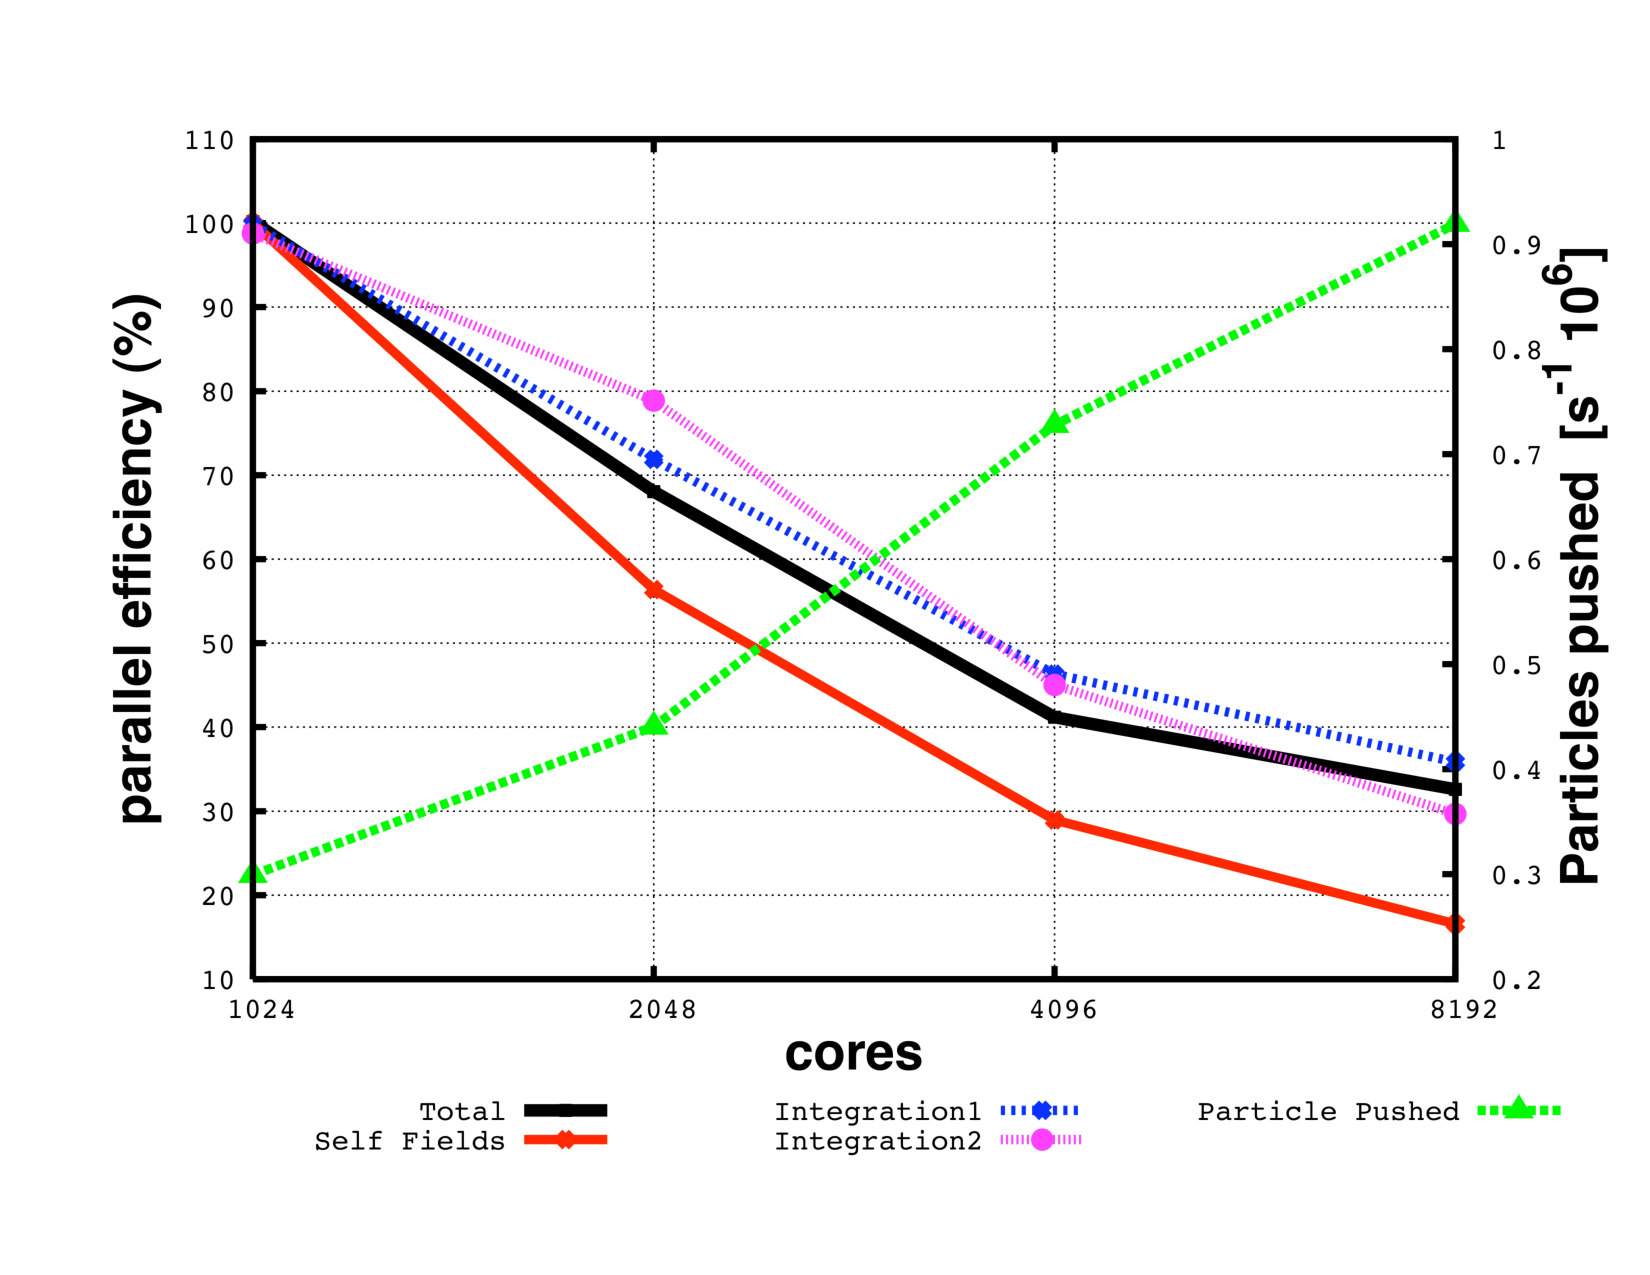
\includegraphics[width=0.75\textwidth]{figures/drift2c1}
\caption{Parallel efficiency and particles pushed per \si{\micro\second} as a function of cores}
\label{fig:walldrift}
\end{figure}
%===========================================================

\section{Quality Management}
Documentation and quality assurance are given our highest attention since we are convinced that adequate documentation
is a key factor in the usefulness of a code like \opal to study present and future particle accelerators.
 Using tools such as a source code version
control system (\href{https://git-scm.com}{git}), source code documentation using Doxygen (found \href{http://amas.web.psi.ch/docs/opal/html/}{here}) and the extensive user manual you are now enjoying, we are committed to providing users as well as co-developers with
state-of-the-art documentation to \opal.

One example of an non trivial test-example is the PSI DC GUN. In \figref{guncomp1} the comparison between \impactt and \opalt is shown. This example is part of the regression test suite
that is run every night. The input file is found in \secref{examplesbeamlines}.

Misprints and obscurity are almost inevitable in a document of this size.
Comments and {\em active contributions}  from readers are therefore most welcome.
They may be sent to \htmladdnormallink{\texttt{andreas.adelmann@psi.ch}}{mailto:andreas.adelmann@psi.ch}.


%======================FIGURE===============================
\begin{figure}[!htb]
\centering
   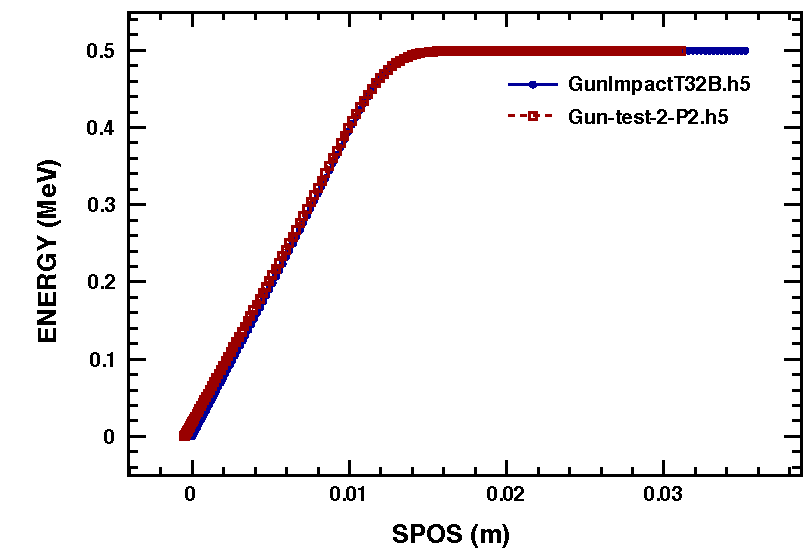
\includegraphics[width=0.45\textwidth]{figures/Gun/GunCompEn}
   \hspace{0.05\textwidth}
   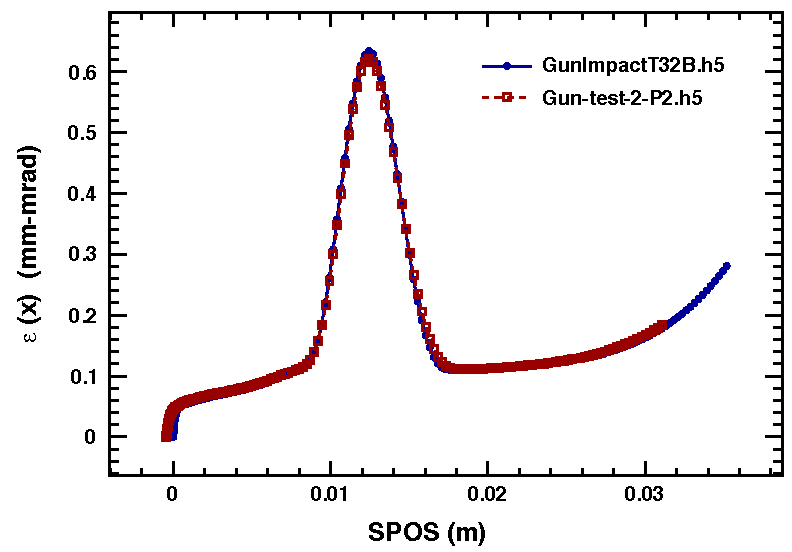
\includegraphics[width=0.45\textwidth]{figures/Gun/GunCompEx}
   \caption{Comparison of energy and emittance in $x$ between \impactt and \opalt}
   \label{fig:guncomp1}
\end{figure}
%===========================================================

\section{Field Maps from the FEMAXX 3D Eigenmode Solver}
\ifthenelse{\boolean{ShowDebug}}{
\TODO{AA will rewrite}

}{}
Electromagnetic field maps for beam dynamics calculations originate from a number of different
electromagnetic solvers, e.g. Superfish and similar codes.

Here, we describe the current status of work in progress which will, eventually,
allow the usage of field maps that have been computed with the FEMAXX $3$-dimensional
electromagnetic eigenmodal solver \cite{bib:arbenzetal2001,bib:arbenzetal2006}.

The FEMAXX code computes electromagnetic eigenmodes of resonant cavities of
arbitrary $3$-dimensional shape and boundary conditions.

Unlike Superfish and similar $2$-dimensional codes, FEMAXX is not restricted in the
kind of geometry it can model. It is therefore possible to consider arbitrary
shapes and their inclusion in beam dynamics and particle tracking calculations.

Given a mesh of a $3$-dimensional geometry FEMAXX computes eigenomdal field
decompositions.

The user then specifies sampling locations for the electromagnetic eigenfields.

At present, sampling locations are specified in terms of a cylinder shape,
i.e. the user indicates the cylinder axis, the radial cylinder vector and
the number of sampling locations in axial, radial and azimuthal directions.

Once the eigenmodal solution has been computed the fields are sampled at
these locations and stored in the T7 file format, for subsequent use in \opal.

Considerable effort has been spent for the validation and benchmarking of
beam dynamics calculations based on T7 field maps computed with FEMAXX.

A pillbox cavity, i.e. a cylinder shape with a radius $r = \SI{4.7}{\centi\meter}$ and
height $h = \SI{3}{\centi\meter}$, has been chosen for benchmarking purposes,
due to the availability of an analytical solution.

The analytical resonance frequency of the dominant mode is \SI{2.441}{\giga\hertz}.


%======================FIGURE===============================
\begin{figure}[!htb]
\centering
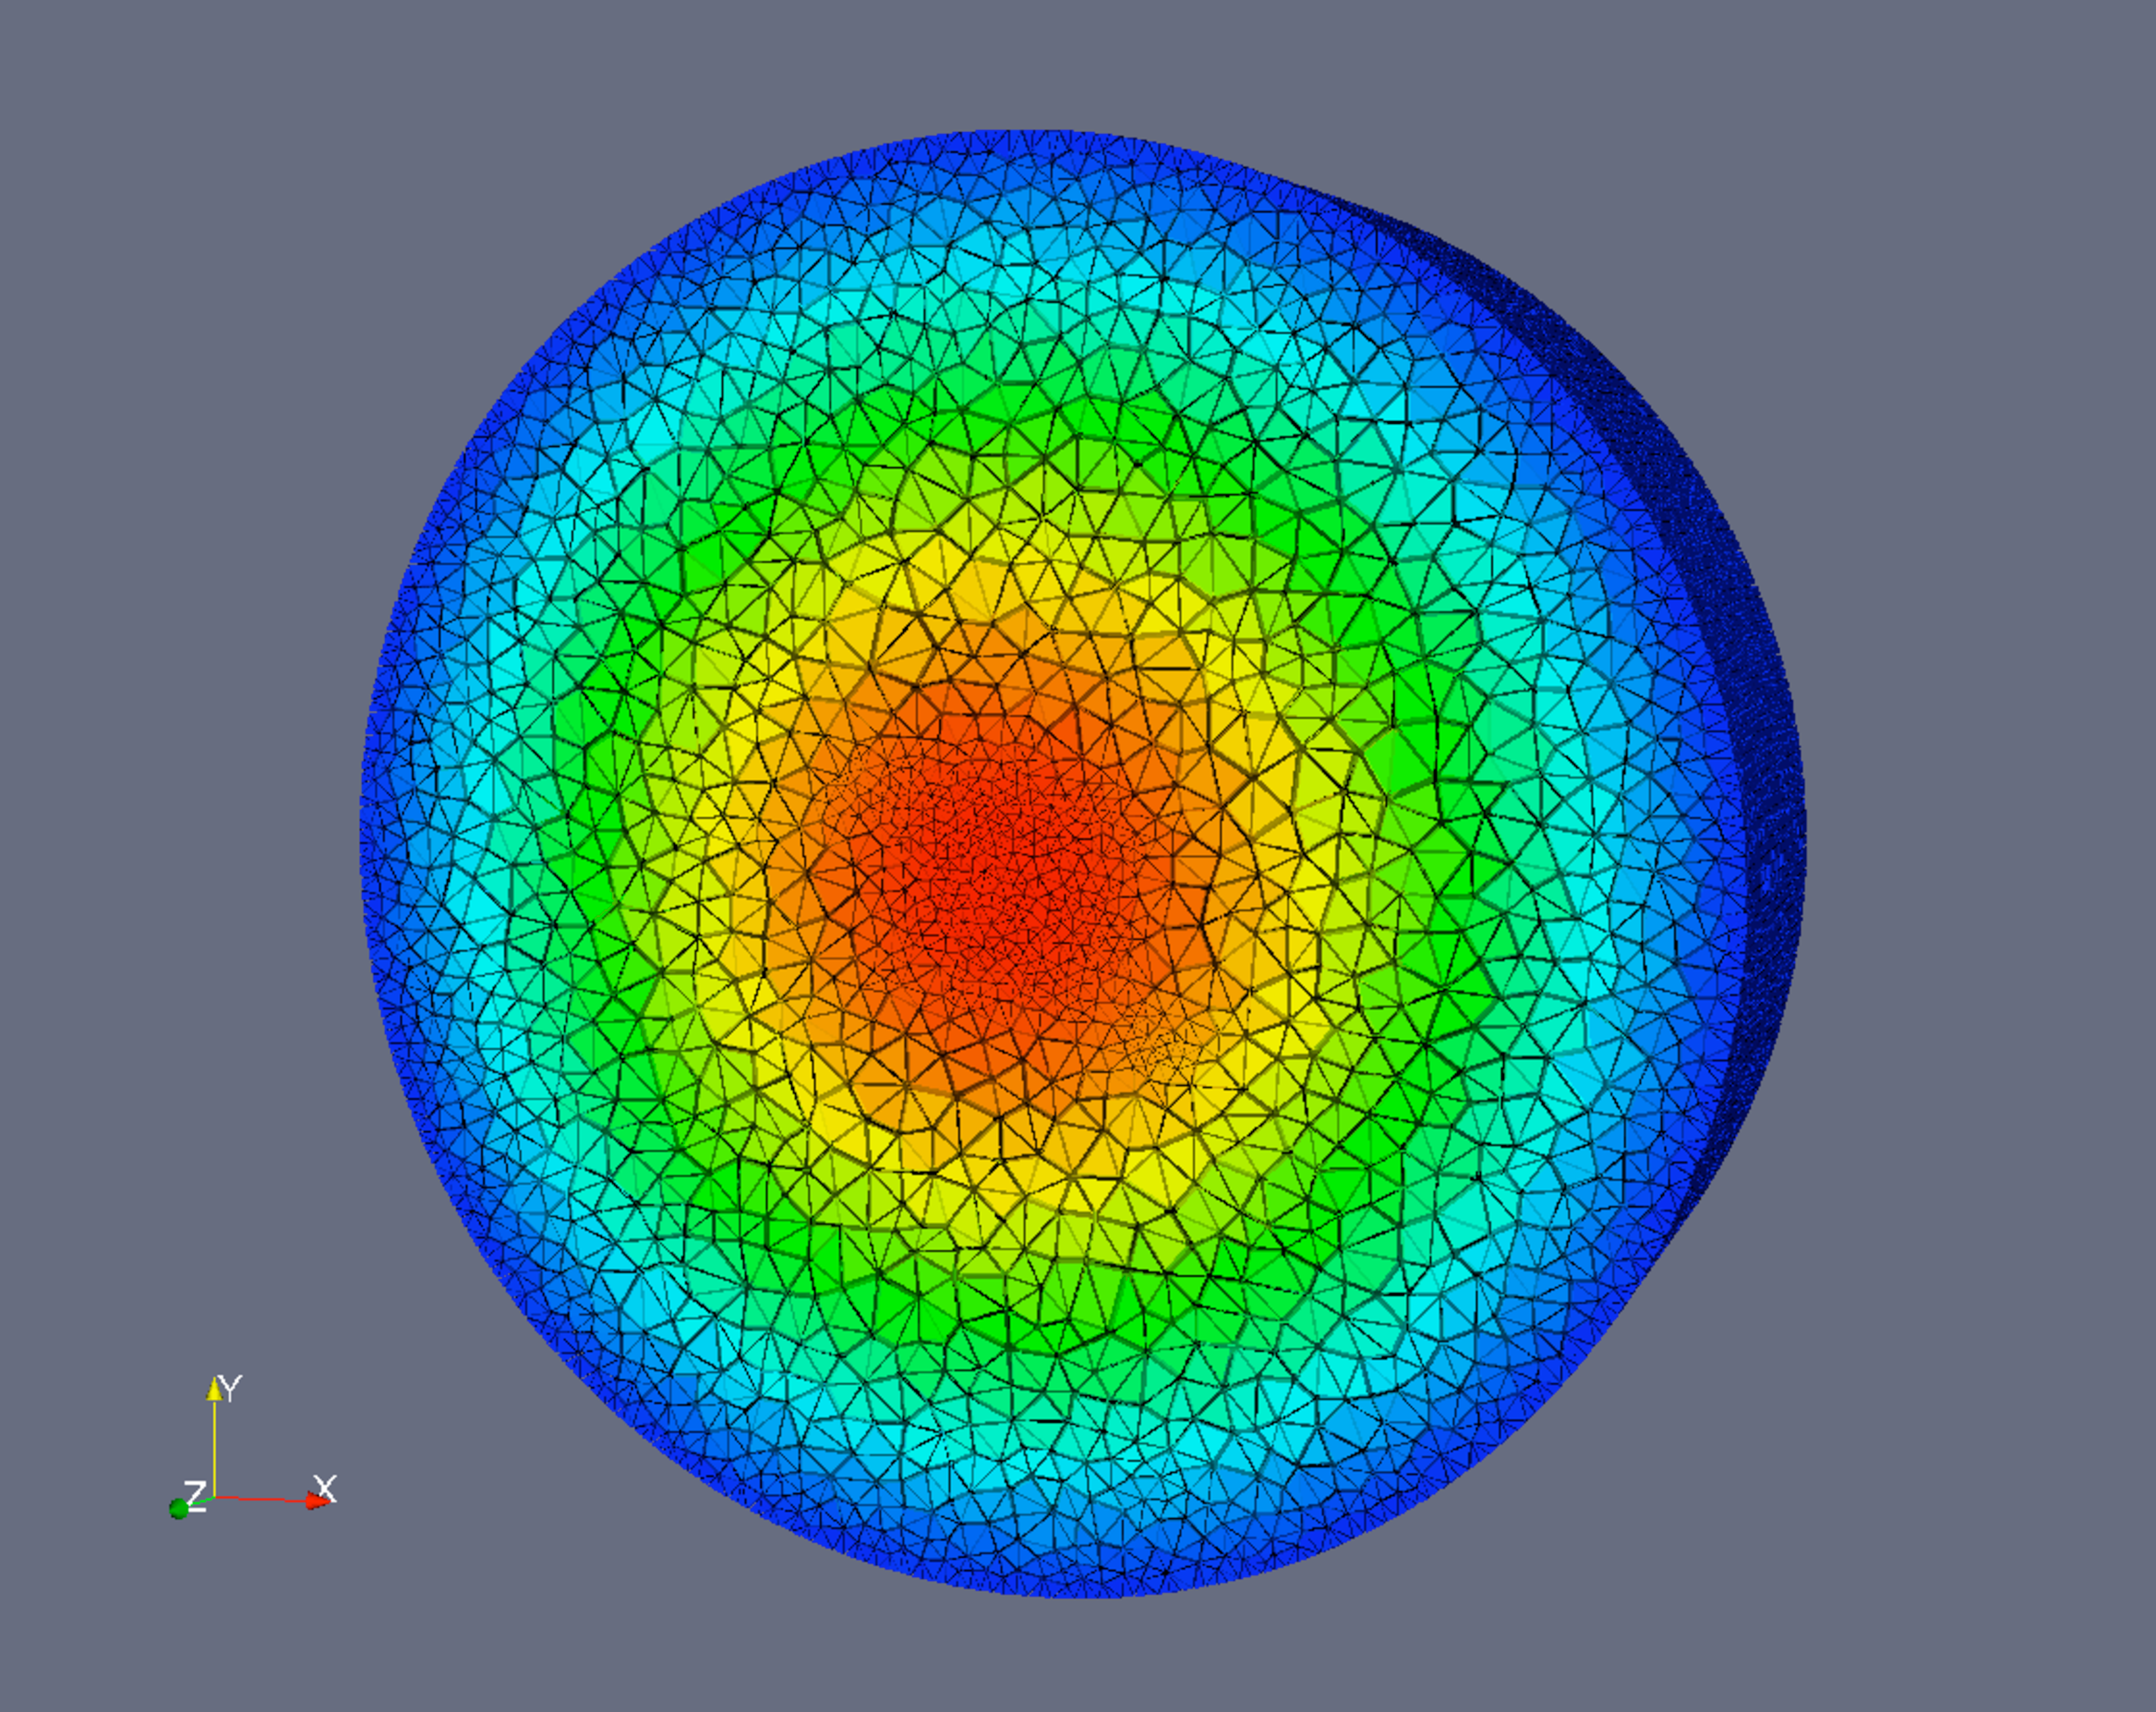
\includegraphics[width=0.6\textwidth]{./figures/adaptivePillboxMesh.pdf}
\caption[Tetrahedral mesh of a pillbox shaped cavity]{We show the discretization of a pillbox shaped cavity geometry into a tetrahedral mesh. The mesh has been adaptively refined so that the region around the cylinder axis is decomposed into smaller tetrahedra than those which are further away from the axis.}
\label{fig:pillbox_adaptively_refined_mesh}
\end{figure}
%===========================================================

We have compared two cases with \opal: (1) The analytical solution has been
sampled within a cylinder volume, stored into a T7 file and used in an \opal
run; (2) the same pillbox shaped geometry has been discretization into tetrahedra
and the eigenmodal fields were calculated with FEMAXX.
%%
These two cases were then compared, resulting in the following conclusions:
%%
(1) Using a relatively coarse mesh with some $110'000$ tetrahedra, the difference
between the analytical and the numerical solution was usually smaller than
$1$ percent.
%%
(2) Using an adaptively refined mesh, the difference between analytical and
numerical solutions decreased below $1$ per mill. The mesh is shown
in \figref{pillbox_adaptively_refined_mesh}.
%%
(3) It is therefore imperative to use a tetrahedral mesh which has been
refined around the beam axis. It is definitely more efficient to use local
refinement, based on physical argument, than simply refine the complete
mesh in a uniform manner.
%%


We are now working towards benchmarking more complicated shapes in order to
assess requirements w.r.t to meshes and modeling geometry so that we
achieve the same or better accuracy as has been obtained from field
maps that were computed with Superfish like solvers based on azimuthal symmetry.


\section{Output}
The phase space is stored in the H5hut file-format \cite{bib:howison2010} and can be analyzed
using e.g. H5root \cite{bib:schietinger}. The frequency
of the data output (phase space and some statistical quantities) can be controlled using the \keyword[sec:option]{OPTION} statement \seesec{option},
 with the flag \keyword{PSDUMPFREQ}. The file is named like in input file but with the extension {\tt .h5}.

A SDDS compatible ASCII file with statistical beam parameters is written to a file with extension {\tt .stat}. The frequency with which this data is written can be controlled with the \keyword[sec:option]{OPTION} statement \seesec{option} with the flag \keyword{STATDUMPFREQ}.
%======================FIGURE===============================
\begin{figure}[!htb]
\centering
 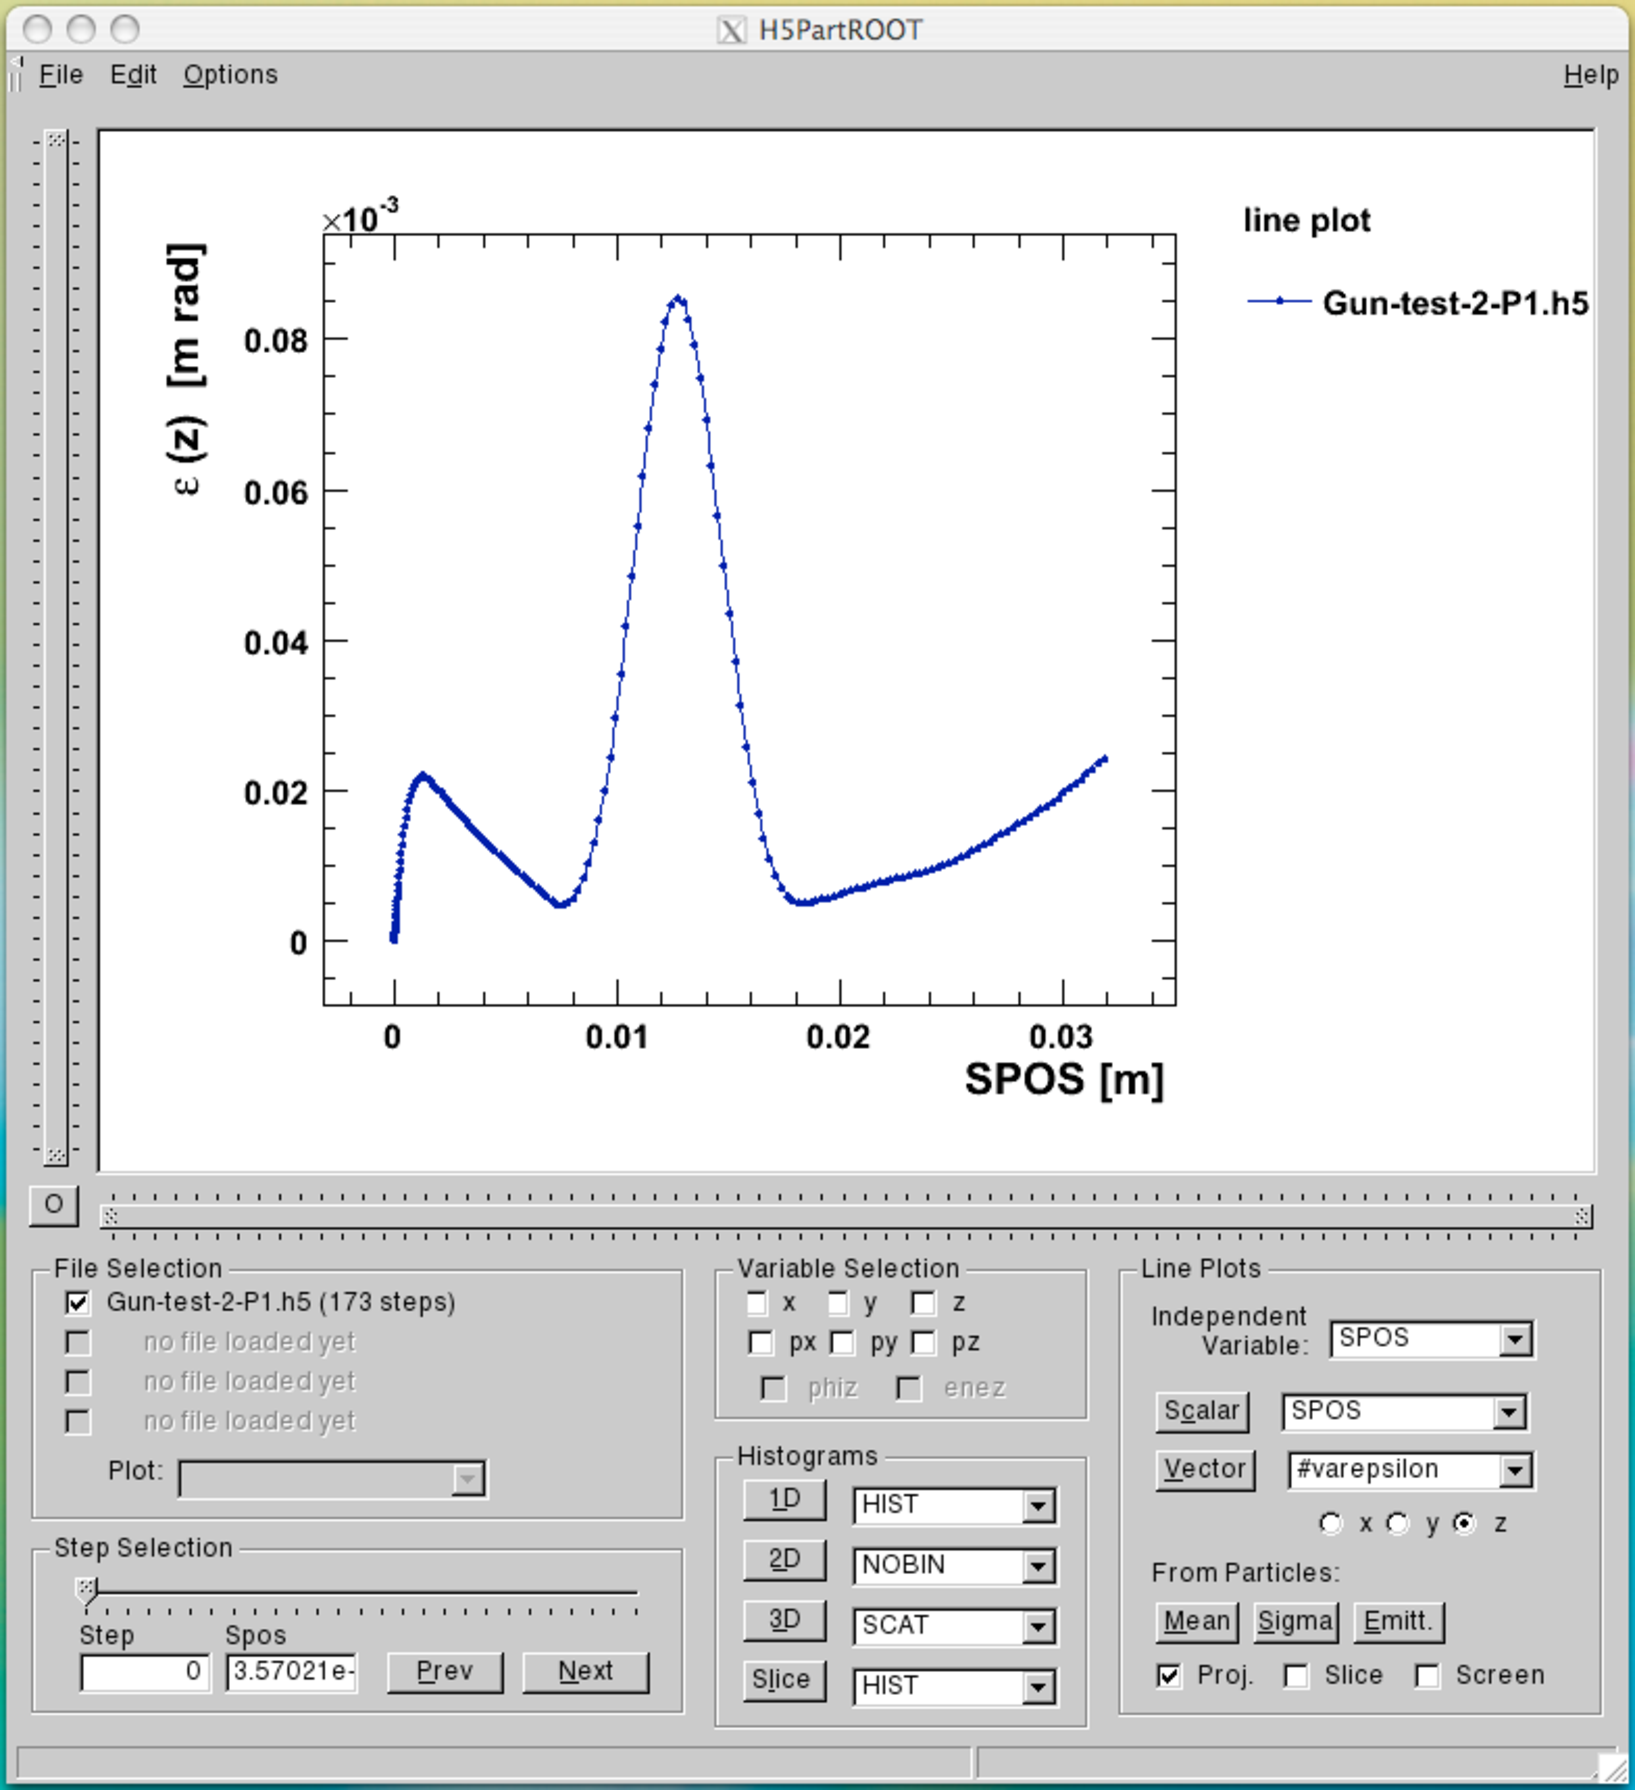
\includegraphics[width=0.32\textwidth]{figures/H5rootPicture1}
 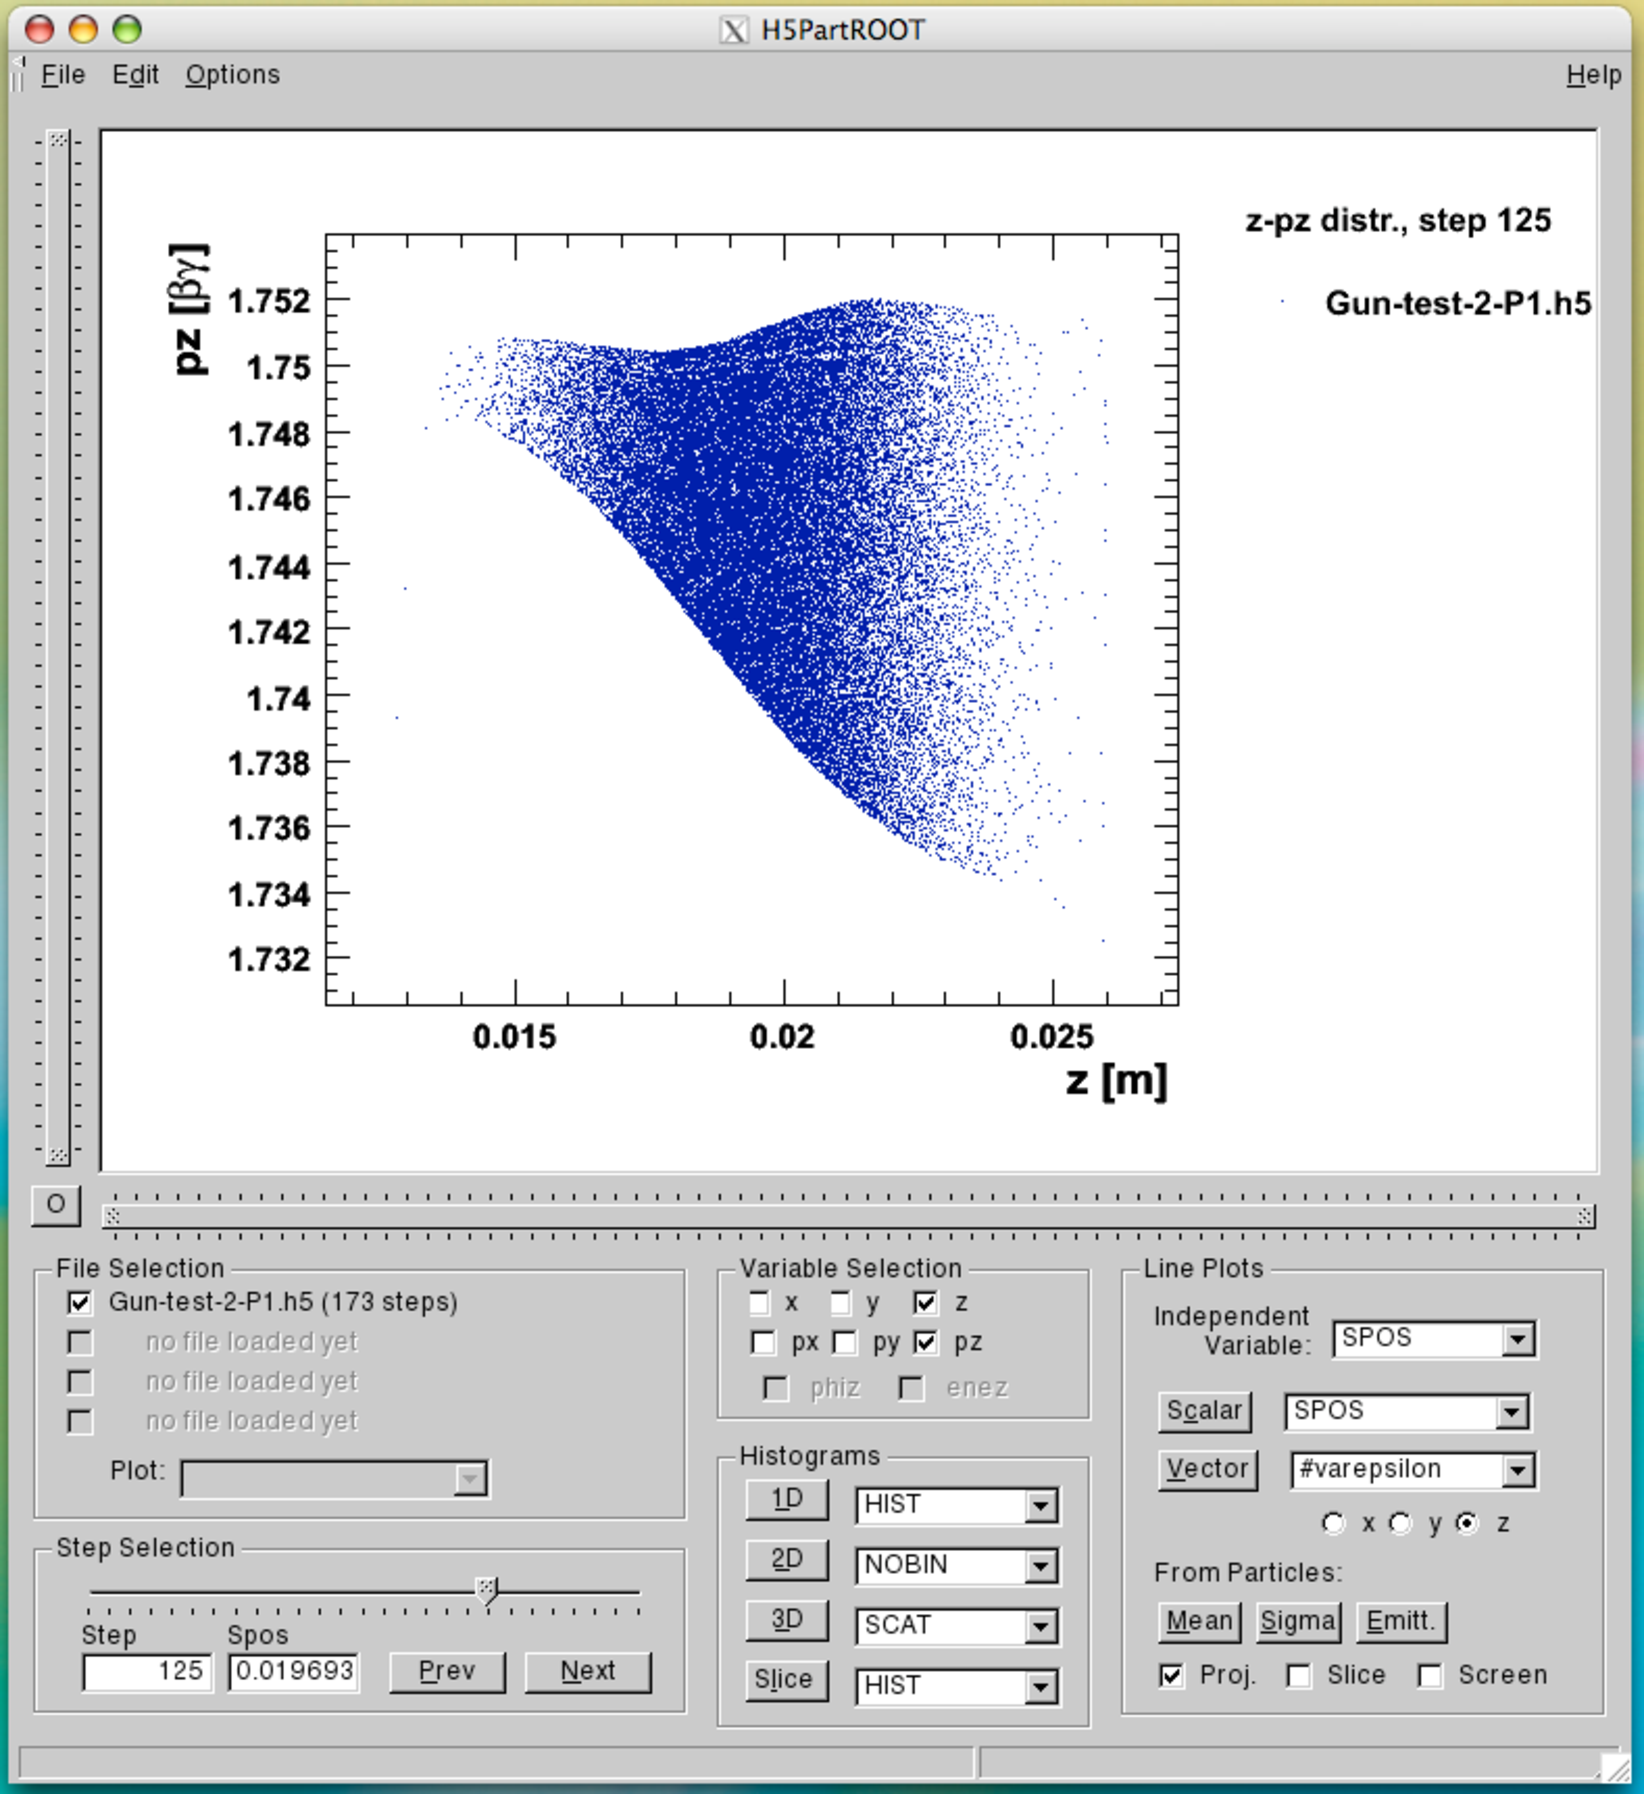
\includegraphics[width=0.32\textwidth]{figures/H5rootPicture2}
 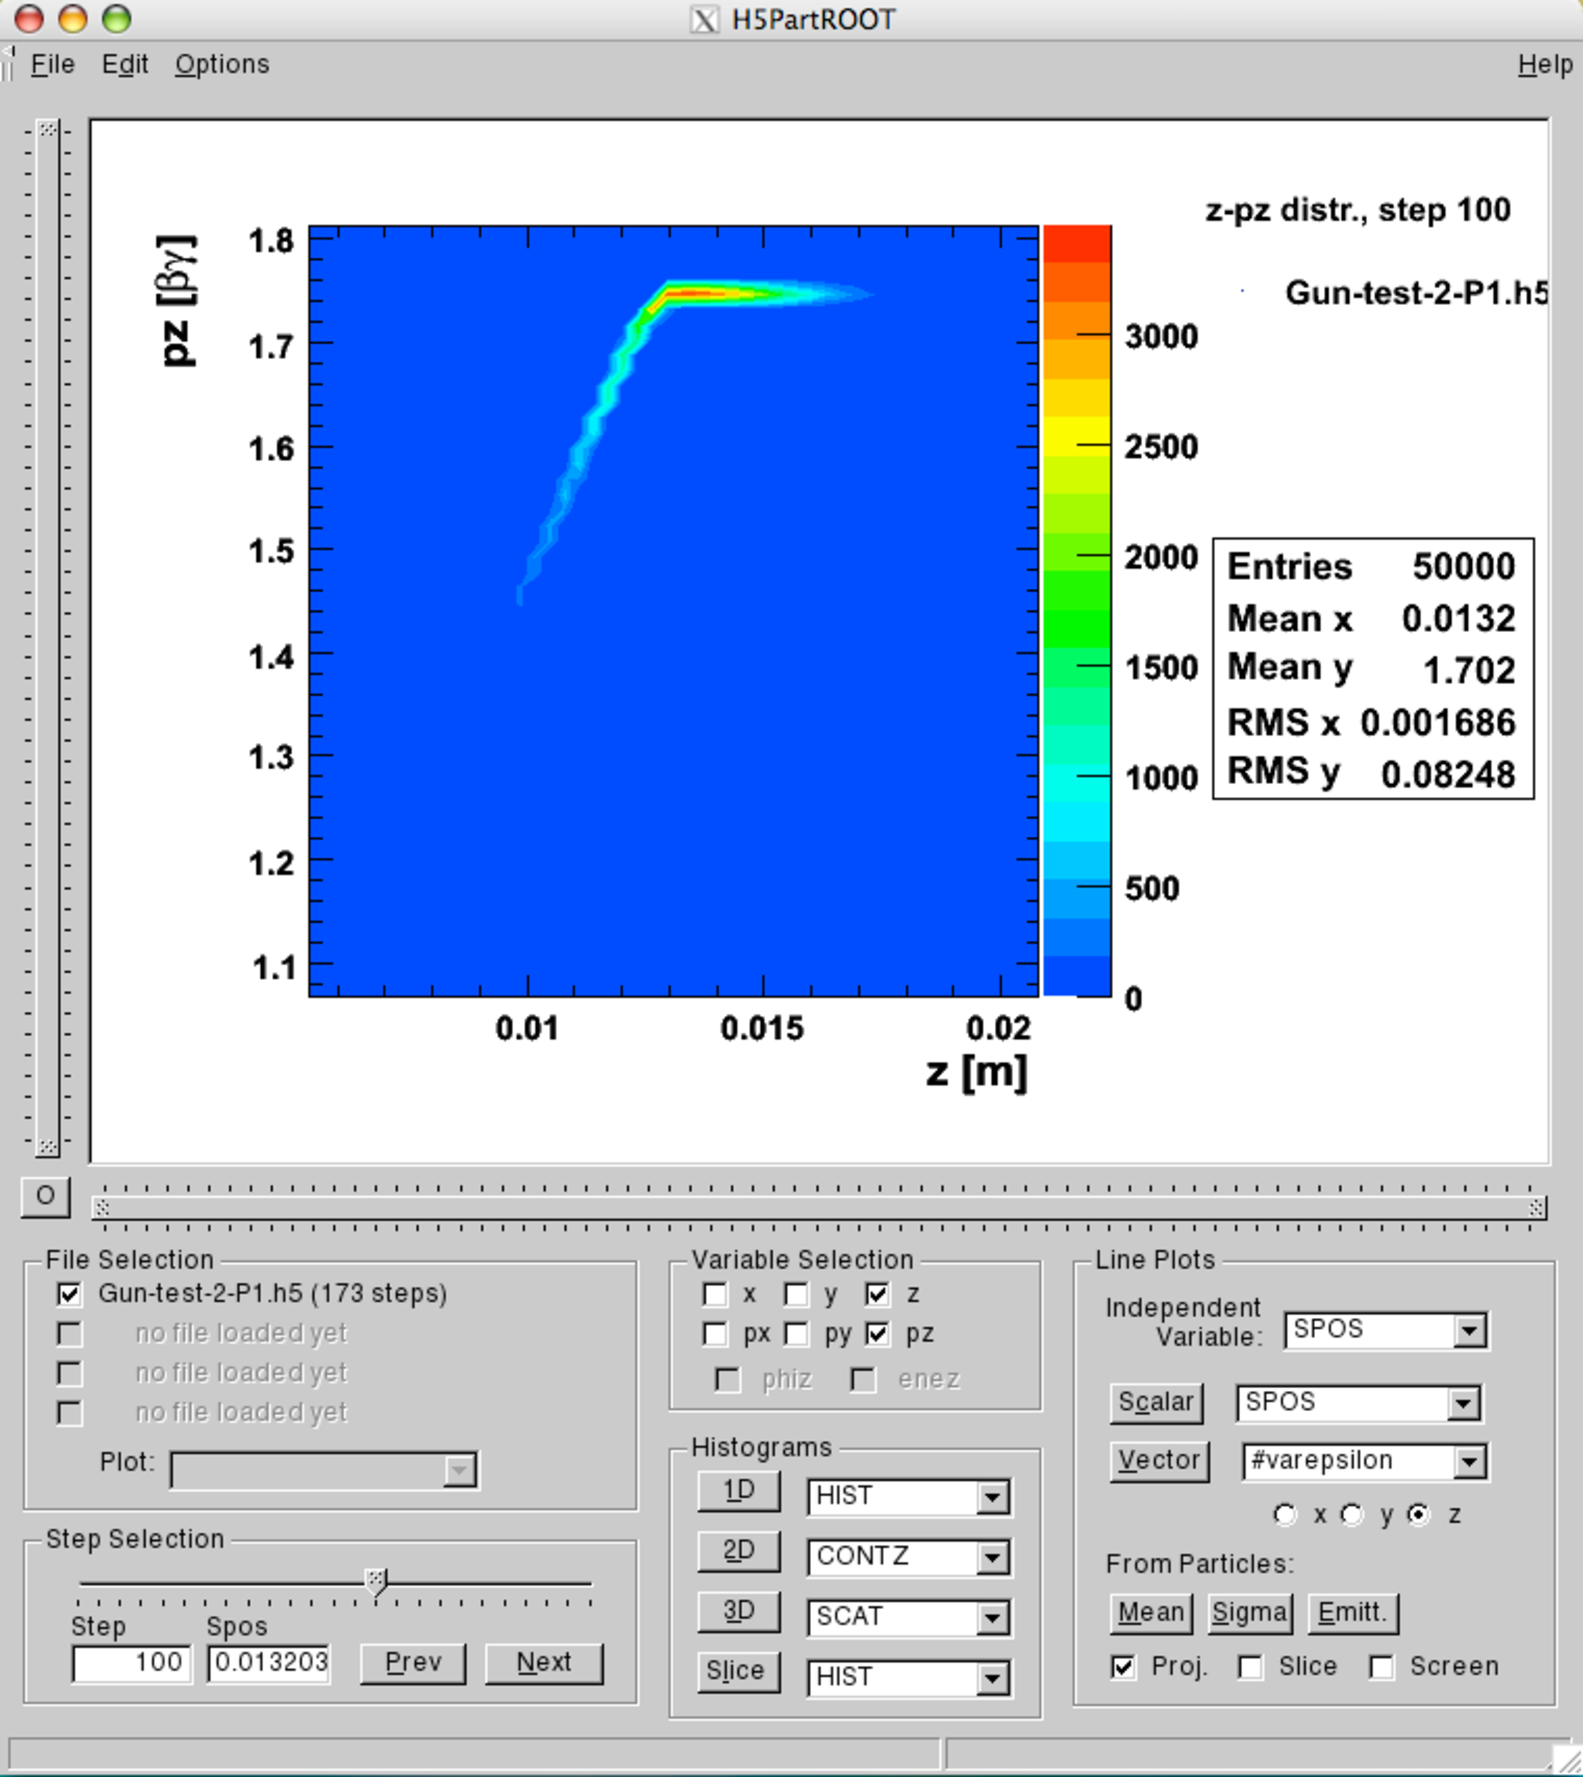
\includegraphics[width=0.31\textwidth]{figures/H5rootPicture3}
\caption[]{H5root enables a variety of data analysis and post processing task on \opal data}
%  \caption{Example of a longitudinal phase space shown with H5root}
 \label{fig:h5root1}
\end{figure}
%===========================================================

\section{Change History}
See \appref{changelog} for a detailed list of changes in \opal.
\section{Known Issues and Limitations}
\subsection{\opalcycl}
\begin{itemize}
    \item Restart with the option \keyword{PSDUMPLOCALFRAME} does not work yet,
    \item In complicated geometries such as spiral inflectors, proper particle deletion at the boundary sometimes fails.
\end{itemize}
\section{Acknowledgments}
The contributions of various individuals and groups are acknowledged in the relevant chapters, however a few individuals have or had considerable influence on the
development of \opal, namely Chris Iselin, John Jowett, Julian Cummings, Ji Qiang, Robert Ryne and Stefan Adam. For the \partroot~ visualization tool credits go to Thomas Schietinger.
The effort to couple FEMAXX to \opal was led by Benedikt Oswald.

The following
individuals are acknowledged for past contributions: Tulin Kaman, Yuanjie Bi, Colwyn Gulliford, Hao Zha and Christopher Mayes.

%- - - - - - - - - - - - - - - SECTION- - - - - - - - - - - - - - - - - - -
\section{Citation}
Please cite \opal in the following way:
\begin{example}
@techreport{opal:1,
title = {The OPAL (Object Oriented Parallel Accelerator Library) Framework},
author = {Andreas Adelmann and Achim Gsell and Valeria Rizzoglio (PSI) and Christof
Metzger-Kraus (HZB) and Yves Ineichen (IBM) and Xiaoying Pang and Steve Russell (LANL)
and Chuan Wang and Jianjun Yang (CIAE) and Suzanne Sheehy and Chris Rogers (RAL) and
Daniel Winklehner (MIT)},
institution = {Paul Scherrer Institut},
number = {PSI-PR-08-02},
year = {(2008-2016)}
}
\end{example}



%----------- Footer control ------------------
\ifthenelse{\boolean{FullOPALManual}}
{
  %do nothing
}
% else (for individual document creation)
{
\appendix
\printbibliography
\end{document}
}
%---------------------------------------------